\documentclass[11pt]{article}
\usepackage[a4paper,margin=28mm]{geometry}
\usepackage{amsmath,amssymb,amsthm,mathtools,booktabs,graphicx}
\usepackage[T1]{fontenc}
\usepackage{lmodern}
\usepackage{microtype}
\usepackage{xurl}
\usepackage[colorlinks=true,linkcolor=black,citecolor=black,urlcolor=black]{hyperref}
\setlength{\emergencystretch}{2em}
\newtheorem{theorem}{Theorem}
\newtheorem{proposition}[theorem]{Proposition}
\newtheorem{lemma}[theorem]{Lemma}
\newtheorem{corollary}[theorem]{Corollary}
\theoremstyle{remark}
\newtheorem{remark}[theorem]{Remark}
\newcommand{\E}{\mathbb E}
\newcommand{\dd}{\,\mathrm d}
\newcommand{\supp}{\operatorname{supp}}
\newcommand{\sgn}{\operatorname{sgn}}
\title{Arbitrarily many population maxima under uniform global dispersal}
\author{Anonymous}
\date{27 October 2026\\[2pt]
\small Version 1.0.0-candidate (unrefereed). DOI: \url{https://doi.org/10.5281/zenodo.23687852}\\
\small Code and data: \url{https://github.com/ipitchford/multiple-dispersal-maxima}}

\begin{document}
\maketitle
\begin{abstract}
How does the total size of a population depend on how often its members
move between habitats of different quality? We study a standard model in
which individuals leave their location at a fixed rate and resettle
anywhere in the habitat with equal probability, as larvae or seeds drawn
from a well-mixed pool do. Bai and Li showed that, when habitat quality
varies by less than a factor of about 1.6, total population has a single
peak as the movement rate changes, and they asked whether several peaks
are possible. We show that they are. A habitat with three quality levels
can give two peaks; two levels never can; and suitably arranged habitats
give any prescribed number of peaks. The mechanism is simple: a tiny
patch of very rich habitat barely changes the average quality but adds
a population bump at a movement rate comparable to its richness. The
result is qualitative. In our explicit examples the extra peaks are very
shallow, and the richest habitat is many times better than the poorest.
We also give an exactly verified three-level example in which the best
habitat is only about 14.2 times better than the worst, against 658 in
our first example.
\end{abstract}

\section{Introduction}

A population spread over a patchy landscape is shaped by two forces.
Local growth pulls each subpopulation towards what its own patch can
support. Movement mixes the subpopulations together. A classical question
in spatial ecology asks how the total equilibrium population depends on
the rate of movement. Two facts are well known: with movement, the total
can exceed the total resource~\cite{Lou2006,DeAngelisNiZhang2016}, and in
two-patch models the total may rise and then fall as dispersal
increases~\cite{FreedmanWaltman1977,ArditiLobrySari2015,GaoLou2022}. In the
model studied here, Bai and Li~\cite{BaiLi2021} proved that the total has
a single peak when habitat quality varies only modestly, and asked whether
it can ever have more than one.

Whether there can be more than one peak matters in practice. If the
response to connectivity has several peaks, a few experiments at one or
two connectivity levels cannot be extrapolated, and the total population
alone cannot identify the dispersal rate. We show that several peaks do
occur, and that there is no upper limit on their number. We also report
how large the effects are. They are mathematically robust but small, and
we say so throughout.

\paragraph{Roadmap.}
Section~\ref{sec:results} states the model and the results.
Section~\ref{sec:scalar} reduces the problem to a single scalar equation.
Section~\ref{sec:two-three} treats two and three resource levels,
including the exact examples and their effect sizes.
Section~\ref{sec:rare} constructs any number of peaks from rare rich
patches, starting with an informal sketch.
Section~\ref{sec:ecology} gives an ecological reading. Section~\ref{sec:related}
places the work in the literature, and Section~\ref{sec:open} lists open
problems.

\section{The model and the results}\label{sec:results}

On the interval \(\Omega=(0,1)\), consider
\begin{equation}\label{eq:model}
 \partial_t u(x,t)=d\bigl(\overline u(t)-u(x,t)\bigr)
                 +u(x,t)\bigl(m(x)-u(x,t)\bigr),
 \qquad
 \overline u(t)=\int_0^1u(x,t)\dd x .
\end{equation}
Here \(u(x,t)\) is the population density at location \(x\). The
\emph{dispersal rate} \(d>0\) is the rate at which individuals leave
their location. Emigrants enter a common pool and settle uniformly over
the habitat, so the immigration rate at every point is \(d\,\overline u\).
The \emph{resource} \(m(x)\) is a bounded function bounded away from zero.
Since the coefficient of \(u^2\) is one everywhere, \(m(x)\) is both the
local intrinsic growth rate and the local carrying capacity. Dispersal
costs nothing in this model.

The unique positive equilibrium is denoted by \(\theta_{m,d}\), and the
total equilibrium population by
\begin{equation}\label{eq:population}
 M_m(d)=\int_0^1\theta_{m,d}(x)\dd x .
\end{equation}
The habitat has measure one, so total population and mean density
coincide. The curve \(d\mapsto M_m(d)\) gives the total population as
connectivity varies.

Equation~\eqref{eq:model} is the uniform nonlocal dispersal model (1.11)
of Bai and Li~\cite{BaiLi2021}. The averaging operator was introduced by
Nagylaki to represent global panmixia~\cite{Nagylaki2011}. Bai and Li's
Theorem~1.5 proves unimodality when
\(\operatorname*{ess\,sup}m/\operatorname*{ess\,inf}m<(1+\sqrt5)/2\approx
1.618\). Next to the question, they note that for perturbations of a
constant the nonlocal model admits exactly one maximum. They then ask
\emph{whether it is possible for the total population to have multiple
maximum points in the model (1.11)}~\cite[Section~5, p.~20]{BaiLi2021}.
We cite their arXiv preprint (version~1); we found no journal version.
Their admissible class allows nonnegative nonconstant resources, so our
positive examples lie inside it.

\begin{theorem}[Arbitrarily many maxima from rare rich patches]\label{thm:main}
Let \(a>0\) and let \(N\geq1\) be an integer. There is a sequence
\(m_j\in C^\infty([0,1])\) with the following properties.
\begin{enumerate}
 \item For every \(j\): \(m_j>0\), \(m_j'(x)>0\) for \(0\leq x\leq1\),
       \(\int_0^1m_j(x)\dd x=a\), and the map \(d\mapsto M_{m_j}(d)\) has at
       least \(N\) distinct strict local maxima in \((0,\infty)\).
 \item As \(j\to\infty\), \(m_j\to a\) in \(L^p(0,1)\) for every
       \(1\leq p<\infty\), but not uniformly. The rich patches shrink in
       area but not in height. In our construction the contrast
       \(\sup m_j/\inf m_j\) exceeds \(2^{N-1}\) for all large \(j\).
\end{enumerate}
\end{theorem}

The theorem should not be read as ``nearly constant habitats can have many
peaks''. Item~2 says only that the heterogeneity occupies a vanishing
area. The pointwise contrast does not shrink, and it grows without bound
in \(N\) in our construction. The population gains between peaks are also
small: they are of order \(\varepsilon\), the area parameter of the rare
patches. All this is consistent with Bai and Li's result for small
pointwise contrast. Monotonicity of \(m_j\) is not a substantive
constraint. Uniform mixing sees only the distribution of resource values
(Section~\ref{sec:scalar}), so any arrangement, including an increasing
one, gives the same curve. Before smoothing, \(N+1\) resource levels
suffice. Here \(C^\infty([0,1])\) means the restriction of a smooth
function defined on a neighbourhood of the closed interval.

\begin{theorem}[An exact three-level example]\label{thm:exact}
Let
\[
 p_1=\frac{2405}{3504},\qquad
 p_2=\frac{1095}{3504}=\frac5{16},\qquad
 p_3=\frac4{3504}=\frac1{876},
\]
and let \(m\) be the increasing step function
\begin{equation}\label{eq:witness}
 m=\tfrac1{20}\ \text{on }(0,p_1),\qquad
 m=\tfrac{25}{12}\ \text{on }(p_1,p_1+p_2),\qquad
 m=\tfrac{329}{10}\ \text{on }(p_1+p_2,1).
\end{equation}
Then
\begin{equation}\label{eq:exact-derivatives}
 M_m(3)=1,\qquad M_m'(3)=0,\qquad
 M_m''(3)=\frac{6042635}{1975192401}>0,
\end{equation}
and \(M_m\) has at least two strict local maxima. Every rearrangement of
\(m\) (every resource with the same distribution of values) has the same
population curve, and so satisfies~\eqref{eq:exact-derivatives} and has
the same two maxima. Moreover, every positive smooth strictly increasing
resource that is sufficiently close in \(L^1(0,1)\) to the increasing step
function~\eqref{eq:witness}, with values in a fixed compact subinterval of
\((0,\infty)\), has a nondegenerate local minimum near \(d=3\) and at least
two distinct strict local maxima. For such approximations the exact
identities~\eqref{eq:exact-derivatives} are not claimed: the location and
value of the minimum move with the resource.
\end{theorem}

\begin{theorem}[Two resource levels]\label{thm:two}
Suppose \(m\) takes the distinct values \(a<b\), on sets of measures
\(p\) and \(q=1-p\), where \(a>0\) and \(0<p<1\). Then
\begin{equation}\label{eq:two-sign}
 \sgn M_m'(d)=\sgn(a+b-2d).
\end{equation}
The unique local and global maximum occurs at \(d=(a+b)/2\), and
\begin{equation}\label{eq:two-max}
 \max_{d>0}M_m(d)
   =\frac{pa+qb+\sqrt{pa^2+qb^2}}2 .
\end{equation}
Among resources taking finitely many values, three is therefore the
smallest number of levels that permits multiple strict local maxima.
\end{theorem}

\begin{proposition}[A low-contrast three-level example]\label{prop:lowcontrast}
Let \(d_0=76/25\) and
\[
 \theta_1=1-10^{-6},\qquad \theta_2=1+10^{-7},\qquad
 \theta_3=\tfrac{57}{5},\qquad
 m_i=\theta_i+d_0-\frac{d_0}{\theta_i}.
\]
The linear system
\(\sum_ip_i=1\), \(\sum_ip_i\theta_i=1\),
\(\sum_ip_i(1-\theta_i)/(\theta_i+d_0/\theta_i)=0\)
has a unique solution, and it is positive. The three-level resource with
values \(m_i\) on sets of measures \(p_i\) satisfies \(M(d_0)=1\),
\(M'(d_0)=0\) and \(M''(d_0)>0\). It therefore has at least two strict
local maxima. Its contrast is
\[
 \frac{m_3}{m_1}=\frac{14173319160000}{999994960001}\approx 14.1734 .
\]
\end{proposition}

So the contrast needed for multiple maxima among three-level resources
lies between Bai and Li's \(1.618\) and the certified \(14.1734\).
Section~\ref{sec:open} records numerical evidence that \(14.17\) is close
to optimal for three levels, and the corresponding open problem. We also
show (Corollary~\ref{cor:finite}) that every critical dispersal rate lies
strictly between the smallest and largest resource values.

\section{Scalar reduction and parameter dependence}\label{sec:scalar}

Uniform global mixing makes the equilibrium population depend only on
the probability distribution \(\mu\) of the resource values, not on
their spatial arrangement. Write \(z\) for a resource value and let
\[
 0<\ell\leq z\leq b<\infty
 \quad\hbox{\(\mu\)-almost everywhere}.
\]
Expectations in this section are with respect to \(\mu\). At equilibrium,
each location balances local growth against the net flow
\(d(M-\theta)\) from the common pool:
\begin{equation}\label{eq:equilibrium}
 d(M-\theta)+\theta(z-\theta)=0,\qquad M=\E\theta .
\end{equation}
For a given pool level \(M\), solving the quadratic gives the local density
\begin{equation}\label{eq:phi}
 \theta=\Phi(z,d,M)
  :=\frac{z-d+\sqrt{(z-d)^2+4dM}}2,
 \qquad
 M=\E\Phi(z,d,M).
\end{equation}
We call the second equation the \emph{closure}. It says that the pool
level must be reproduced by averaging the local densities it induces.

\begin{lemma}[Existence, uniqueness and analytic dependence]\label{lem:scalar}
For every \(d>0\), equation~\eqref{eq:phi} has a unique positive solution
\(M=M_\mu(d)\). It satisfies
\[
 \ell\leq M\leq b,\qquad
 \ell\leq \Phi(z,d,M)\leq b.
\]
The function \(M_\mu\) is real analytic on \((0,\infty)\).
If
\begin{equation}\label{eq:A-D}
 A=2\theta+d-z=\theta+\frac{dM}{\theta},
 \qquad D=1-d\E\frac1A,
\end{equation}
then
\begin{equation}\label{eq:D-positive}
 D=\frac1M\E\frac{\theta^2}{A}>0.
\end{equation}
\end{lemma}

In words, \(A\) is the local stiffness: \(1/A\) measures how strongly the
density at a site responds to a change in its inflow. The quantity \(D\)
is the stabilising factor of the closure. It is the derivative of
\(M-\E\Phi\) with respect to \(M\), and its positivity drives every
implicit-function step below.

\begin{proof}
For fixed \(z,d\), differentiating~\eqref{eq:phi} in \(M\) gives
\(\Phi_M=d/A\). The identity
\[
 \Phi-M\Phi_M=\frac{\Phi^2}{A}>0
\]
shows that \(\E\Phi(z,d,M)/M\) is strictly decreasing in \(M>0\).
At \(M=\ell\), every integrand \(\Phi(z,d,\ell)\) is at least
\(\ell\), whereas at \(M=b\) every integrand \(\Phi(z,d,b)\) is at
most \(b\). Continuity therefore gives a root in \([\ell,b]\);
strict decrease of the quotient gives uniqueness among all positive
roots. The density bounds follow because the positive root of the
quadratic lies between \(z\) and \(M\).

Averaging the displayed identity at a root proves~\eqref{eq:D-positive}.
The map \(F(d,M)=\E\Phi(z,d,M)-M\) is real analytic near every
\((d,M)\in(0,\infty)^2\). Indeed, the discriminant is bounded away
from zero on a sufficiently small common neighbourhood, uniformly for
\(z\in[\ell,b]\), and the resulting convergent power series can be
integrated term by term. At a root, \(F_M=-D<0\).
The analytic implicit function theorem proves the assertion.
\end{proof}

Direct substitution into~\eqref{eq:equilibrium} gives, for \(c>0\), the
\emph{scaling law}
\begin{equation}\label{eq:scaling}
 M_{cm}(d)=c\,M_m(d/c).
\end{equation}
Only the ratio of dispersal rate to resource level matters. Multiplying
all resources by \(c\) moves every peak from \(d_*\) to \(cd_*\) and
leaves the number and strictness of peaks unchanged.

\begin{lemma}[Population excess and endpoint limits]\label{lem:endpoints}
Let \(\bar m=\E z\). If \(\mu\) is not concentrated at one point, then
\begin{equation}\label{eq:excess}
 M_\mu(d)>\bar m\quad(d>0),\qquad
 \lim_{d\downarrow0}M_\mu(d)
 =\lim_{d\to\infty}M_\mu(d)=\bar m.
\end{equation}
For every resource distribution,
\begin{equation}\label{eq:moment-bound}
 M_\mu(d)\leq\frac{\E z+\sqrt{\E z^2}}2.
\end{equation}
\end{lemma}

The inequality \(M_\mu>\bar m\) is the phenomenon in which total population
exceeds total carrying capacity~\cite{Lou2006,DeAngelisNiZhang2016}.
For this model it holds at every dispersal rate.

\begin{proof}
Dividing~\eqref{eq:equilibrium} by \(\theta\) and averaging yields
\[
 M-\bar m=d\left(M\E\frac1\theta-1\right)\geq0,
\]
by Jensen's inequality. The inequality is strict unless \(\theta\) is
constant almost surely; the equilibrium equation then makes \(z\) constant
as well. The small-\(d\) limit follows uniformly from~\eqref{eq:phi} and
\(\ell>0\). For the other limit, the uniform density bounds and
\eqref{eq:equilibrium} give \(\theta-M=O(d^{-1})\).
Averaging~\eqref{eq:equilibrium} gives
\(\E\theta(z-\theta)=0\), and thus
\(M(\bar m-M)=O(d^{-1})\). Since \(M\geq\bar m>0\), the limit follows.
Finally,
\(\E(\theta-z/2)^2=\E z^2/4\) by the same identity. Cauchy--Schwarz,
applied to the mean of \(\theta-z/2\), proves~\eqref{eq:moment-bound}.
\end{proof}

\begin{lemma}[Continuity under resource approximation]\label{lem:continuity}
Let \(m_k,m:(0,1)\to[\ell,b]\), where \(0<\ell<b<\infty\), and suppose
\(\|m_k-m\|_{L^1}\to0\). On every compact interval
\(I=[d_0,d_1]\subset(0,\infty)\),
\[
 M_{m_k}\longrightarrow M_m\quad\hbox{in }C^2(I).
\]
In particular, any finite collection of strict inequalities between
population values at prescribed dispersal rates in \(I\) is preserved for
sufficiently large \(k\). So are strict sign conditions on \(M'\) and
\(M''\) on \(I\).
\end{lemma}

The full \(C^2\) statement is used only in the smoothing step of
Theorem~\ref{thm:exact}. The other applications need only the preservation
of strict inequalities between values.

\begin{proof}
The root function obeys
\[
 0<\Phi_z=\frac{\Phi}{2\Phi+d-z}<1.
\]
Consequently \(|\E_{m_k}\Phi-\E_m\Phi|\le\|m_k-m\|_{L^1}\) for every
\((d,M)\): the closure functions converge uniformly in \((d,M)\). All
their positive roots belong to \([\ell,b]\). Compactness, continuity and
the uniqueness in Lemma~\ref{lem:scalar} imply uniform convergence of the
roots for \(d\in I\). Otherwise a sequence \(d_k\to d_*\) and a convergent
subsequence of roots would give a second positive root at \(d_*\).

On the compact set \(K=I\times[\ell,b]\), the derivatives of \(\Phi\) in
\((d,M)\) through order three are smooth functions of \(z\in[\ell,b]\),
with uniformly bounded \(z\)-derivatives. Their expectations under \(m_k\)
therefore converge to those under \(m\), uniformly on \(K\). Using
\(\ell\le\theta,M\le b\) and \(A=\theta+dM/\theta\le b+d_1b/\ell\), we get
the uniform lower bound
\begin{equation}\label{eq:D-lower}
 D=\frac1M\E\frac{\theta^2}{A}\ \ge\ \frac{\ell^2}{b\,(b+d_1b/\ell)}>0
 \qquad (d\in I),
\end{equation}
for every resource with values in \([\ell,b]\). The implicit formulas
\(M'=\E[\Phi_d]/D\) and
\(M''=\bigl(\E[\Phi_{dd}+2\Phi_{dM}M'+\Phi_{MM}(M')^2]\bigr)/D\),
where \(D=1-\E\Phi_M\), are continuous in these expectations and in
\(1/D\). This gives the asserted \(C^2\) convergence.
\end{proof}

\begin{remark}[Strictness from analyticity]\label{rem:trapping}
If \(0<d_-<d_0<d_+\) and
\[
 M(d_0)>\max\{M(d_-),M(d_+)\},
\]
then \(M\) attains a maximum on \([d_-,d_+]\) at an interior point. The
trap forces \(M\) to be nonconstant on \((d_-,d_+)\), so by analyticity it
is nonconstant on \((0,\infty)\). A nonconstant real analytic function has
only isolated critical points, so this maximum is strict. Traps whose open
intervals \((d_-,d_+)\) are disjoint therefore give distinct strict local
maxima, even when two traps share an endpoint. This lets us work with
finitely many population values, without a numerical root count for
\(M'\).
\end{remark}

\section{Two and three resource levels}\label{sec:two-three}

Differentiating~\eqref{eq:equilibrium} gives
\begin{equation}\label{eq:derivative}
 A\theta'=M-\theta+dM',
 \qquad
 M'=\frac{\E[(M-\theta)/A]}{D}.
\end{equation}
The numerator has a useful pairwise representation. For independent
resource values \(z,\widetilde z\), put
\(\theta=\Phi(z,d,M)\), \(\widetilde\theta=\Phi(\widetilde z,d,M)\)
and define \(\widetilde A\) correspondingly. Then
\begin{align}
 \E\frac{M-\theta}{A}
 &=\frac12\E\left[
   \frac{(\theta-\widetilde\theta)^2}{A\widetilde A}
       \left(1-\frac{dM}{\theta\widetilde\theta}\right)\right]\notag\\
 &=\frac12\E\left[
 \frac{(\theta-\widetilde\theta)^2(z+\widetilde z-2d)}
      {(\theta+\widetilde\theta)A\widetilde A}\right].
 \label{eq:pairwise}
\end{align}
The first equality is the standard two-copy expression for a covariance.
The second uses
\[
 z+\widetilde z-2d
  =(\theta+\widetilde\theta)
      \left(1-\frac{dM}{\theta\widetilde\theta}\right).
\]
Each pair of resource values pushes the population up when the dispersal
rate is below their average, and down when it is above.

\begin{proof}[Proof of Theorem~\ref{thm:two}]
Let \(x<y\) be the equilibrium densities at resources \(a<b\).
Formula~\eqref{eq:pairwise} reduces to
\[
 \E\frac{M-\theta}{A}
   =\frac{pq(y-x)^2(a+b-2d)}{(x+y)A_xA_y}.
\]
Every factor except \(a+b-2d\) is positive. This proves
\eqref{eq:two-sign}. At the unique critical rate \(d_*=(a+b)/2\),
the pairwise identity gives \(d_*M=xy\).
Subtracting the two resource equations then gives
\(y-x=(b-a)/2=:\Delta\).
The relations \(M=x+q\Delta\) and \(d_*M=x(x+\Delta)\) give
\(x^2-ax-d_*q\Delta=0\), and \(a^2+4d_*q\Delta=pa^2+qb^2\), so
\[
 x=\frac{a+\sqrt{pa^2+qb^2}}2.
\]
Adding \(q\Delta\) proves~\eqref{eq:two-max}. A one-level resource gives a
constant curve, and Theorem~\ref{thm:exact} gives two maxima with three
levels. This proves the minimality statement for finitely-valued resources.
\end{proof}

\begin{corollary}[Each fixed resource has finitely many critical rates]
\label{cor:finite}
Let a positive bounded nonconstant resource have essential infimum
\(\ell>0\) and essential supremum \(b\). Then \(M'(d)>0\) for
\(0<d\leq\ell\) and \(M'(d)<0\) for \(d\geq b\). Its critical rates form a
finite subset of \((\ell,b)\).
\end{corollary}

\begin{proof}
The signs follow directly from~\eqref{eq:pairwise}. Nonconstancy gives
strictness even at the two endpoints. Analyticity and the nonzero
endpoint signs exclude infinitely many zeros of \(M'\) in the compact
interval \([\ell,b]\).
\end{proof}

At a stationary population value, differentiating the first equation
in~\eqref{eq:derivative} once more, using \(A'=2\theta'+1\) and
\(\E\theta''=M''\), yields
\begin{equation}\label{eq:second}
 D M''=-2\E\frac{(\theta')^2+\theta'}{A},
 \qquad \theta'=\frac{M-\theta}{A}.
\end{equation}

\paragraph{How the examples are found.}
The weights in Theorem~\ref{thm:exact} look arbitrary, but they are
easy to construct. Fix \(d\) and \(M=1\) and choose the equilibrium
densities \(\theta_i\) first. Equation~\eqref{eq:equilibrium} then gives
the resources, \(m_i=\theta_i+d-dM/\theta_i\). The three conditions
\(\sum p_i=1\), \(\sum p_i\theta_i=1\) and \(M'(d)=0\) are linear in the
habitat fractions \(p_i\). It remains to check that the \(p_i\) are
positive and that~\eqref{eq:second} gives \(M''>0\). Theorem~\ref{thm:exact}
uses \(d=3\) and \(\theta=(4/5,4/3,30)\).

\begin{proof}[Proof of Theorem~\ref{thm:exact}]
At \(d=3\), the equilibrium values, their \(A\)-values, and their
derivatives at a stationary mean are
\[
\begin{array}{c@{\qquad}c@{\qquad}c}
 \toprule
 \theta_i&A_i&\theta_i'\\
 \midrule
 4/5&91/20&4/91\\
 4/3&43/12&-4/43\\
 30&301/10&-290/301\\
 \bottomrule
\end{array}
\]
Indeed \(\sum_i p_i\theta_i=1\), and
\(m_i=\theta_i+3-3/\theta_i\), which verifies all equilibrium equations
exactly. Also,
\[
 \sum_i\frac{p_i}{A_i}=\frac5{21},\qquad
 \sum_i p_i\frac{1-\theta_i}{A_i}=0.
\]
Thus \(D=2/7\) and \(M'(3)=0\). The remaining exact expectation is
\[
 \sum_i p_i\frac{(\theta_i')^2+\theta_i'}{A_i}
   =-\frac{6042635}{13826346807}.
\]
Formula~\eqref{eq:second} gives~\eqref{eq:exact-derivatives}. Since \(M\)
depends only on the distribution of values, the same holds for every
rearrangement of \(m\).

\emph{Two maxima.} Since \(d=3\) is a strict local minimum, there are
points \(d_-<3<d_+\) arbitrarily close to \(3\) with
\(M(d_\pm)>M(3)=1\). By~\eqref{eq:excess}, \(M(d)\to\bar m=347/480<1\) as
\(d\downarrow0\) and as \(d\to\infty\). Hence \(M\) attains a maximum
on \((0,3)\) and another on \((3,\infty)\), each at an interior point.
The traps \((\alpha,d_-,3)\) and \((3,d_+,\gamma)\), for suitable
\(\alpha<d_-\) and \(\gamma>d_+\), share the endpoint \(3\) but have disjoint
open intervals, so the two maxima are distinct. Both are strict by
Remark~\ref{rem:trapping}.

\emph{Smooth increasing versions.} Extend the increasing step function
\(m\) of~\eqref{eq:witness} constantly beyond the endpoints, convolve it
with a nonnegative smooth mollifier, and add \(\kappa x\) with \(\kappa\downarrow0\).
The resulting functions are positive, smooth and strictly increasing,
take values in \([1/20,329/10+1]\), and converge to \(m\) in \(L^1\).
(Spatial \(L^1\) approximation by increasing functions requires this
increasing arrangement; it is not possible for an arbitrary arrangement.)
Choose a closed interval \(I\ni3\) on which \(M''>0\), with \(M'\) negative
at its left endpoint and positive at its right endpoint.
Lemma~\ref{lem:continuity} gives \(C^2\) convergence on \(I\), so every
sufficiently close approximant \(\tilde m\) with values in the fixed range
has a nondegenerate local minimum \(d_{\tilde m}\in I\), where
\(M_{\tilde m}(d_{\tilde m})\) is close to, but in general not equal
to,~\(1\). (A sequential statement becomes the neighbourhood statement of
the theorem by the usual argument by contradiction.) Each approximant is nonconstant, so
Lemma~\ref{lem:endpoints} gives \(M_{\tilde m}>\int\tilde m\) everywhere,
with both endpoint limits equal to \(\int\tilde m\), which is close to
\(\bar m<1\) and hence below \(M_{\tilde m}(d_{\tilde m})\). The argument of
the previous paragraph, with \(3\) replaced by \(d_{\tilde m}\), then gives
two distinct strict local maxima.
\end{proof}

\begin{proof}[Proof of Proposition~\ref{prop:lowcontrast}]
The method is the one just described, with \(d=76/25\). Solving the
\(3\times3\) linear system in exact rational arithmetic gives
\(p_1,p_2,p_3>0\). Then \(\sum p_i\theta_i=1\) and each equilibrium equation
hold exactly, so \(M(d_0)=1\) by the uniqueness in Lemma~\ref{lem:scalar}.
The third equation is \(M'(d_0)=0\) by~\eqref{eq:derivative}. The exact
values of \(D>0\) and of the expectation in~\eqref{eq:second} give
\(M''(d_0)>0\). The exact values, computed and asserted in rational
arithmetic by \path{contrast_witness.py} and recorded in
\path{contrast_witness.json}, are
\[
 p_3=\frac{3570001575000175}{480662491691127955758767000019}
   \approx7.43\times10^{-15},
\]
\[
 D=\frac{549999325000133}{2221997272999905}\approx0.2475,
\]
with \(p_1\approx0.0909092\), \(p_2\approx0.9090908\), and
\(M''(d_0)=-2S/D\), where \(S\) is the expectation in~\eqref{eq:second},
equals a positive rational with a \(52\)-digit numerator and a
\(73\)-digit denominator,
\(M''(d_0)\approx1.0797588\times10^{-21}\).
Because the curvature is so small, we also give a check that does not use
\(M''\). By Lemma~\ref{lem:scalar}, the closure \(F(d,M)=\E\Phi(m,d,M)-M\)
is positive for \(M<M(d)\) and negative for \(M>M(d)\), so the sign of
\(F(d,1)\) is the sign of \(M(d)-1\). Rigorous rational enclosures of the
square roots in \(\Phi\) (script \path{interval_traps.py}, standard library
only) certify
\[
 M(d_0-10^{-4})<1,\quad M(d_0-10^{-5})>1,\quad
 M(d_0+10^{-2})>1,\quad M(\tfrac{31}{10})<1,
\]
while \(M(d_0)=1\) exactly. So \((d_0-10^{-4},\,d_0-10^{-5},\,d_0)\) and
\((d_0,\,d_0+10^{-2},\,\tfrac{31}{10})\) are traps with disjoint open
intervals, and Remark~\ref{rem:trapping} gives two strict local maxima
directly.
Lemma~\ref{lem:endpoints} applies because the law is nonconstant. Every
nonconstant law satisfies \(M>\bar m\) and has endpoint limits \(\bar m\),
so the two-maxima argument in the proof of Theorem~\ref{thm:exact} applies
without change.
\end{proof}

\begin{figure}[t]
 \centering
 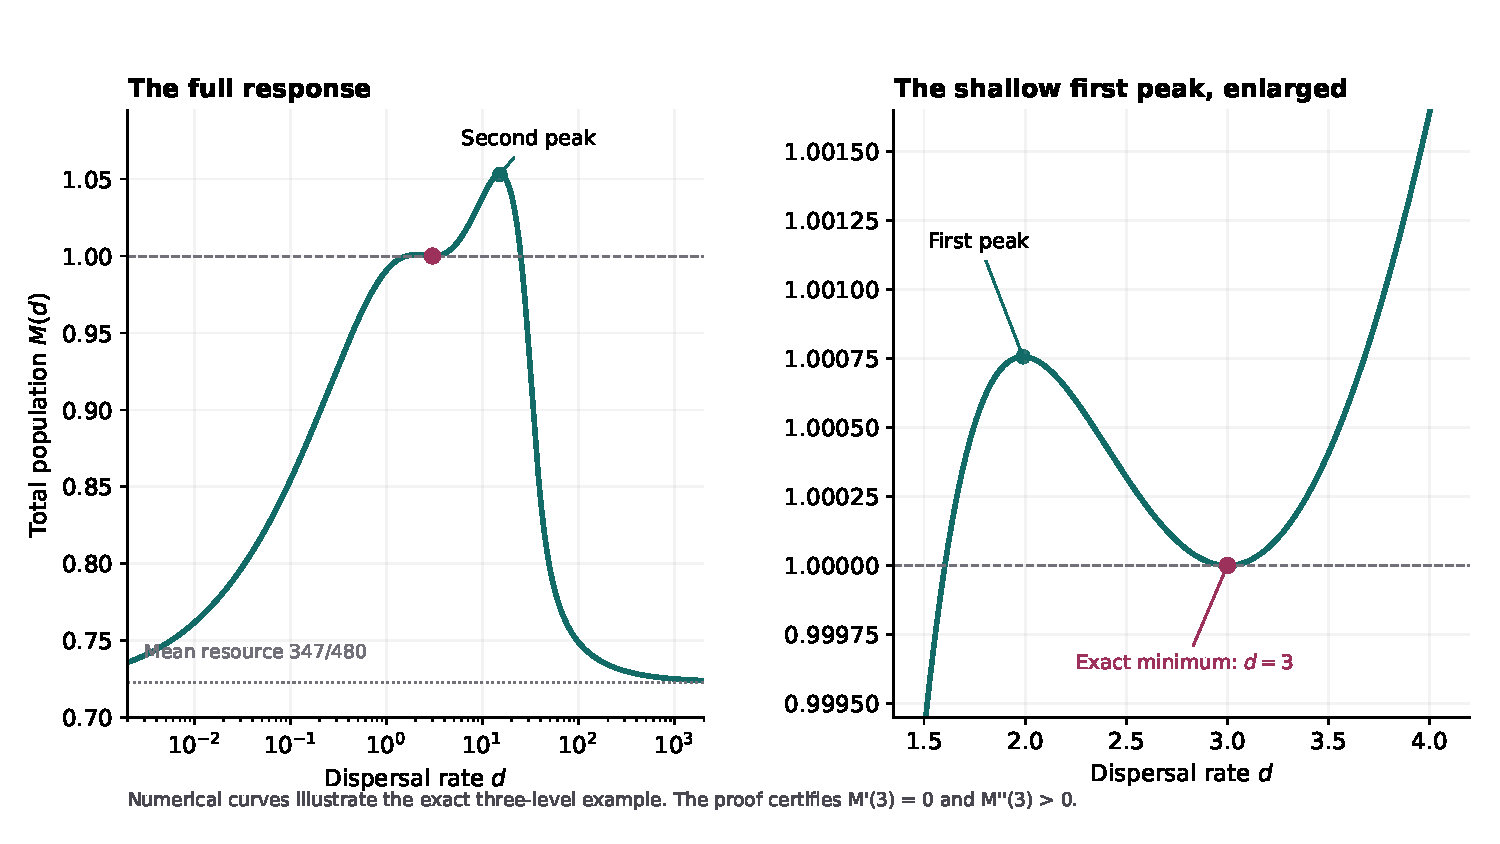
\includegraphics[width=\textwidth]{three_level_population.pdf}
 \caption{The exact three-level example of Theorem~\ref{thm:exact}. Left:
 the full response on a logarithmic dispersal axis. Right: the shallow
 first maximum, enlarged. The minimum at \(d=3\) is certified by
 \eqref{eq:exact-derivatives}. The plotted curves and the marked maxima
 are computed numerically: the maxima by Brent's method on \(M'\), in the
 script that draws the figure. They illustrate the result but are not used
 in the proof.}
 \label{fig:exact}
\end{figure}

\paragraph{Effect sizes.}
Figure~\ref{fig:exact} shows how fragile the first example is.
Numerically, the first maximum is at \(d\approx1.989\) with
\(M\approx1.000756\). The certified minimum is at \(d=3\) with \(M=1\). The
second maximum is at \(d\approx15.08\) with \(M\approx1.0530\). The first
peak rises only about \(7.6\times10^{-4}\) above the minimum, a relative
depth of about \(0.08\%\). This is why the right panel enlarges it. The
contrast is \(m_3/m_1=658\), and the richest level occupies \(1/876\) of
the habitat. Table~\ref{tab:effects} compares the two exact examples.
The low-contrast example of Proposition~\ref{prop:lowcontrast} buys its
contrast with an even shallower dip: \(M''(d_0)\) is of order
\(10^{-21}\), and the rich patch has area about \(7\times10^{-15}\).
This example is quantitatively extremely fragile. Its left maximum lies
within \(10^{-4}\) of \(d_0\) and rises only about \(10^{-32}\) above
\(M(d_0)=1\); its right maximum lies in \((d_0+10^{-2},\,3.1)\). The
witness sits at the edge of the feasible three-level region: changing
\(d_0\) to \(3.03\), \(\theta_3\) to \(11.3\), \(\theta_2\) to \(1+10^{-6}\) or
\(\theta_1\) to \(1-10^{-7}\) makes \(M''(d_0)\) negative, and the two maxima
of this construction disappear. The existence claim is nevertheless
rigorous, because the certificate is exact. Both examples are
qualitative. They show that multiple maxima exist, not that they would be
visible in a census.

\begin{table}[t]
\centering
\caption{Effect sizes of the exact examples (maxima located numerically;
minima certified exactly).}
\label{tab:effects}
\begin{tabular}{lcc}
\toprule
 & Theorem~\ref{thm:exact} & Proposition~\ref{prop:lowcontrast}\\
\midrule
Contrast \(\max m/\min m\) & \(658\) & \(\approx14.1734\)\\
Area of richest level & \(1/876\) & \(\approx7\times10^{-15}\)\\
Certified minimum & \(d=3\), \(M=1\) & \(d=3.04\), \(M=1\)\\
\(M''\) at the minimum & \(\approx3.06\times10^{-3}\) & \(\approx1.08\times10^{-21}\)\\
First maximum & \(d\approx1.989\), \(M\approx1.000756\) & not resolved in double precision\\
Second maximum & \(d\approx15.08\), \(M\approx1.0530\) & not resolved in double precision\\
Relative depth of first dip & \(\approx7.6\times10^{-4}\) (0.08\%) & not resolved in double precision\\
\bottomrule
\end{tabular}
\end{table}

\section{The response to rare resource patches}\label{sec:rare}

\paragraph{The idea in brief.}
Start from a constant habitat with resource \(a\). Replace a tiny fraction
\(\varepsilon w\) of it with very rich habitat of resource \(r\). The mean
resource barely changes, but the population gains an extra amount
\(\varepsilon w\,g_r(d)\), where \(g_r\) is an explicit positive bump in
the dispersal rate. It vanishes at very small and very large \(d\) and
peaks near \(d\approx r/2\) (Lemma~\ref{lem:scales}). Now use several rich
levels \(r_1\ll r_2\ll\cdots\ll r_N\), each rarer than the last. The
bumps sit at widely separated dispersal rates and barely interfere, so
their sum has \(N\) separate humps (Figure~\ref{fig:kernels}). For small
\(\varepsilon\) the true population is the mean resource plus
\(\varepsilon\) times this sum, up to an error of order \(\varepsilon^2\),
so it inherits the \(N\) humps. Smoothing and rescaling then give
Theorem~\ref{thm:main}.

Fix a background resource \(a>0\). For a resource level \(r\ne a\), define
\begin{equation}\label{eq:kernel}
 t_r(d)=\Phi(r,d,a),\qquad
 g_r(d)=\frac{d(t_r(d)-a)^2}{a\,t_r(d)}.
\end{equation}
Here \(t_r(d)\) is the density a site of resource \(r\) would reach if the
pool were held at the background level \(a\). The kernel \(g_r\) is the
first-order population gain above the mean resource when a small part of
a constant habitat is replaced by resource \(r\).

\begin{lemma}[First variation in patch abundance]\label{lem:variation}
Let \(r_1,\ldots,r_k\ne a\) be positive and \(w_1,\ldots,w_k>0\), and put
\[
 W=\sum_{i=1}^kw_i,\qquad
 \mu_\varepsilon=(1-\varepsilon W)\delta_a
                +\varepsilon\sum_{i=1}^kw_i\delta_{r_i},
 \quad 0\le\varepsilon<W^{-1}.
\]
Let \(a_\varepsilon=\int z\dd\mu_\varepsilon(z)\). For every compact
interval \(I=[d_0,d_1]\subset(0,\infty)\) there are \(\varepsilon_I>0\) and
\(C_I<\infty\) such that
\begin{equation}\label{eq:first-variation}
 \Bigl|M_{\mu_\varepsilon}(d)-a_\varepsilon
   -\varepsilon\sum_{i=1}^kw_i g_{r_i}(d)\Bigr|\le C_I\varepsilon^2
 \qquad(d\in I,\ 0\le\varepsilon\le\varepsilon_I).
\end{equation}
\end{lemma}

\begin{proof}
For this finite atomic law the closure is
\[
 F(\varepsilon,d,M)=(1-\varepsilon W)\Phi(a,d,M)
 +\varepsilon\sum_iw_i\Phi(r_i,d,M)-M=0,
\]
which is jointly real analytic in \((\varepsilon,d,M)\) on a neighbourhood
of \(\{0\}\times I\times\{a\}\), even for small negative \(\varepsilon\).
At \(\varepsilon=0\) the root is \(M=a\), and
\(F_M=-D=-a/(a+d)\le-a/(a+d_1)<0\) uniformly on \(I\). The analytic
implicit function theorem gives, near each \(d\in I\), an analytic root
\(M(\varepsilon,d)\). By continuity and compactness of \(I\) there are
\(\delta>0\) and \(\varepsilon_I\in(0,1/(2W))\) such that
\(F_M\le-a/(2(a+d_1))<0\) whenever \(|M-a|\le\delta\),
\(|\varepsilon|\le\varepsilon_I\) and \(d\in I\). On this set \(F\) is
strictly decreasing in \(M\), so it has at most one root there. The local
implicit-function solutions therefore agree on overlaps, and together they
define one analytic function \(M(\varepsilon,d)\) on
\([-\varepsilon_I,\varepsilon_I]\times I\). The choice
\(\varepsilon_I<1/(2W)\) keeps \(1-\varepsilon W>0\), so \(\mu_\varepsilon\) is a
probability law for \(0\le\varepsilon\le\varepsilon_I\).
For \(\varepsilon\ge0\) it coincides with \(M_{\mu_\varepsilon}(d)\) by the
uniqueness in Lemma~\ref{lem:scalar}. Differentiating \(F=0\) in
\(\varepsilon\) at \(\varepsilon=0\), using \(\Phi(a,d,a)=a\) and
\(\Phi_M=d/(a+d)\) there, gives
\[
 \left.\frac{\partial M}{\partial\varepsilon}\right|_{\varepsilon=0}
 =\frac{a+d}{a}\sum_iw_i(t_{r_i}(d)-a).
\]
Since \(a_\varepsilon=a+\varepsilon\sum_iw_i(r_i-a)\), the coefficient of
\(\varepsilon\) in \(M-a_\varepsilon\) is the weighted sum of
\(\frac{a+d}{a}(t_r-a)-(r-a)\). Using \(r=t_r+d-da/t_r\), this equals
\(d(t_r-a)(1/a-1/t_r)=g_r(d)\). Taylor's theorem in \(\varepsilon\), with
\(C_I=\tfrac12\max|\partial_\varepsilon^2M|\) over the compact set
\([0,\varepsilon_I]\times I\), gives~\eqref{eq:first-variation} uniformly
in \(d\in I\).
\end{proof}

\begin{lemma}[Separated scales]\label{lem:scales}
For each fixed \(r\ne a\), \(g_r(d)>0\) for \(d>0\), and
\[
 \lim_{d\downarrow0}g_r(d)=\lim_{d\to\infty}g_r(d)=0.
\]
As \(R\to\infty\),
\begin{align}
 R^{-2}g_R(d)&=O(R^{-1})\longrightarrow0
                 &&\text{for every fixed }d>0,\label{eq:fixed-scale}\\
 R^{-2}g_R(sR)&\longrightarrow\frac{s(1-s)}a
                 &&\text{for }0<s<1,\label{eq:peak-scale}\\
 R^{-2}g_R(R)&\longrightarrow0.\label{eq:end-scale}
\end{align}
\end{lemma}

\begin{proof}
The root \(t_r\) lies strictly between \(a\) and \(r\), so positivity
is immediate. The first endpoint limit follows from \(t_r(0)=r\).
For \(d\to\infty\), the equilibrium identity gives
\(t_r-a=t_r(r-t_r)/d=O(d^{-1})\), and hence \(g_r(d)=O(d^{-1})\).
For fixed \(d\), \(t_R(d)/R\to1\), so \(g_R(d)=O(R)\).
For \(0<s<1\), the quadratic formula gives
\[
 \frac{t_R(sR)}R
   =\frac{1-s+\sqrt{(1-s)^2+4sa/R}}2\longrightarrow1-s.
\]
Substitution into~\eqref{eq:kernel} proves~\eqref{eq:peak-scale}.
Finally \(t_R(R)=\sqrt{aR}\), and substitution proves~\eqref{eq:end-scale}.
\end{proof}

\begin{lemma}[Positive sums with any prescribed number of humps]
\label{lem:many-kernels}
For every \(N\geq1\), there are
\[
 a<r_1<\cdots<r_N,\qquad r_{k+1}>2r_k,
\]
and \(N\) pairwise disjoint intervals
\([\alpha_j,\gamma_j]\subset(0,\infty)\), containing points
\(\alpha_j<\beta_j<\gamma_j\), for which the function
\begin{equation}\label{eq:G}
 G_N(d)=\sum_{i=1}^N r_i^{-2}g_{r_i}(d)
\end{equation}
satisfies
\begin{equation}\label{eq:traps}
 G_N(\beta_j)>
       \max\{G_N(\alpha_j),G_N(\gamma_j)\},
 \qquad j=1,\ldots,N.
\end{equation}
\end{lemma}

\begin{proof}
We construct the resource levels inductively, starting with \(G_0=0\)
and no intervals, with the convention \(r_0:=a\). Suppose \(G_k\) and its \(k\) strict trapping
inequalities have been chosen. Since \(G_k(d)\to0\) as
\(d\to\infty\), choose \(L>r_k\) larger than all right endpoints chosen
so far, with \(G_k(L)<1/(16a)\). For \(R\) larger than all chosen resource
levels, define
\[
 G_{k+1}(d)=G_k(d)+R^{-2}g_R(d).
\]
At each of the finitely many old trapping points, the added term
tends to zero by~\eqref{eq:fixed-scale}, so the old inequalities
survive for all sufficiently large \(R\). Moreover, using
Lemma~\ref{lem:scales} and the decay at infinity of the finitely many old
kernels,
\[
 G_{k+1}(L)\longrightarrow G_k(L)<\frac1{16a},\qquad
 G_{k+1}(R/2)\longrightarrow\frac1{4a},\qquad
 G_{k+1}(R)\longrightarrow0 .
\]
Hence, for all sufficiently large \(R>2L\), we have
\(G_{k+1}(L)<1/(8a)\), \(G_{k+1}(R/2)>3/(16a)\) and
\(G_{k+1}(R)<1/(16a)\). So the triple \((L,R/2,R)\) is a new strict trap,
disjoint from all the old ones. Set \(r_{k+1}=R\), which exceeds
\(2L>2r_k\), and continue.
\end{proof}

\begin{figure}[t]
 \centering
 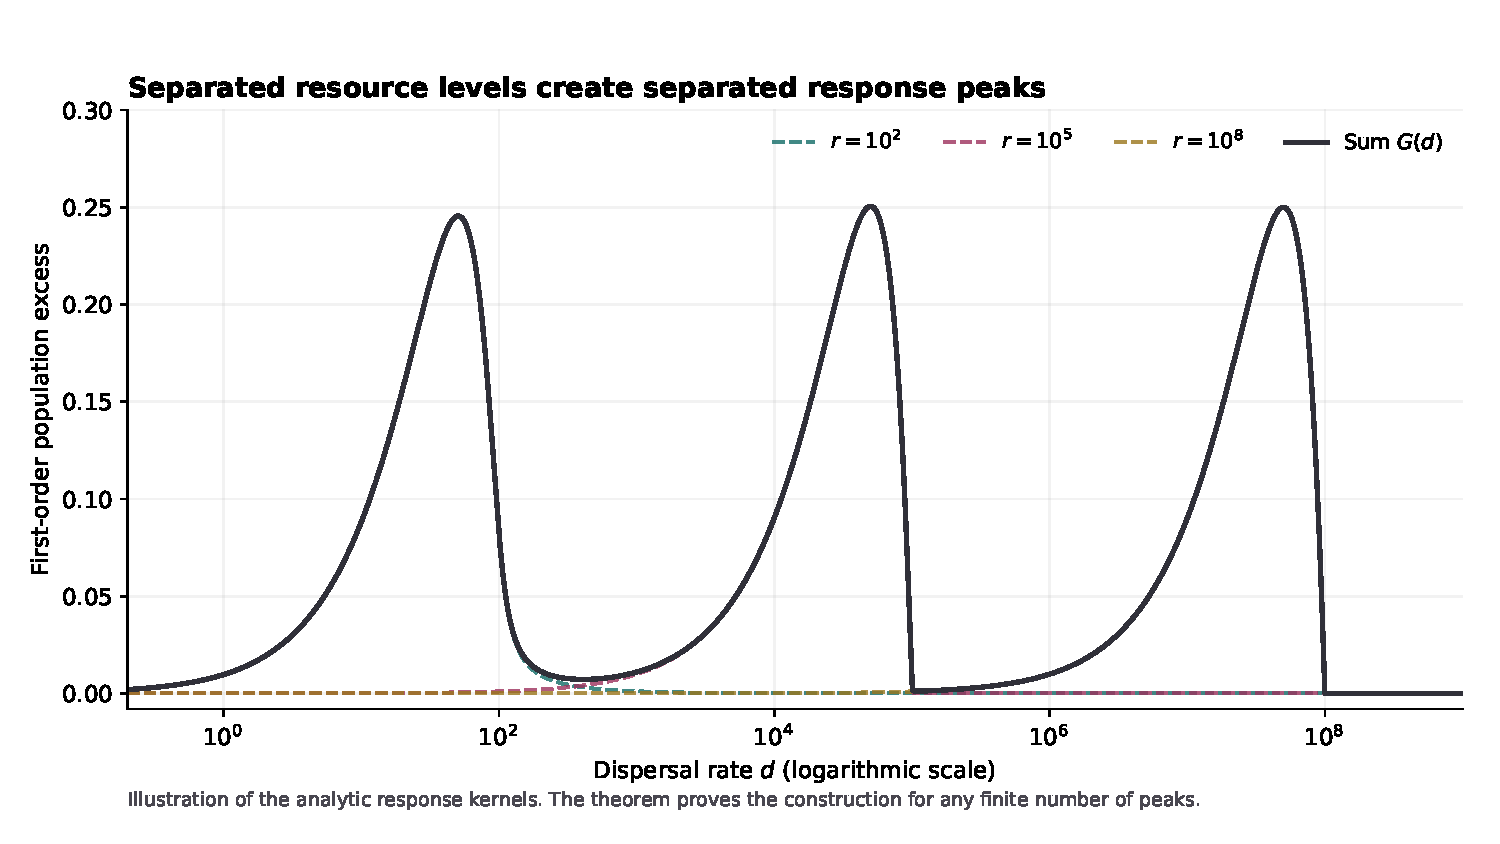
\includegraphics[width=\textwidth]{separated_response_kernels.pdf}
 \caption{The first-variation construction with background \(a=1\),
 resource levels \(10^2,10^5,10^8\) and weights \(r_i^{-2}\). The curve
 shown is the kernel sum \(G_N\), not the nonlinear population
 \(M_{\mu_\varepsilon}\). The true population excess is \(\varepsilon\)
 times this curve, so its vertical scale is small.
 Lemma~\ref{lem:variation} transfers strict inequalities from this sum to
 the nonlinear equilibrium for all sufficiently small \(\varepsilon>0\).}
 \label{fig:kernels}
\end{figure}

\begin{proof}[Proof of Theorem~\ref{thm:main}]
\emph{Step 1: atomic laws.} Take the levels and the \(3N\) trapping points
from Lemma~\ref{lem:many-kernels}, and let \(I\) be a compact interval
containing all of them. Let \(\Delta>0\) be the smallest margin in
\eqref{eq:traps}. Apply Lemma~\ref{lem:variation} on \(I\) with
\(w_i=r_i^{-2}\). Since \(a_\varepsilon\) does not depend on \(d\), every
difference \(M_{\mu_\varepsilon}(\beta_j)-M_{\mu_\varepsilon}(\alpha_j)\)
equals \(\varepsilon(G_N(\beta_j)-G_N(\alpha_j))\) up to \(2C_I\varepsilon^2\),
and similarly at \(\gamma_j\). So for
\(0<\varepsilon<\varepsilon_*:=\min\{\varepsilon_I,\Delta/(4C_I)\}\), each
of the \(N\) traps holds for \(M_{\mu_\varepsilon}\) with margin at least
\(\varepsilon\Delta/2\). The traps lie in disjoint intervals, so
Remark~\ref{rem:trapping} gives \(N\) distinct strict local maxima. The
law \(\mu_\varepsilon\) has \(N+1\) levels, including the background
\(a\).

\emph{Step 2: smoothing, with the tolerance chosen after \(\varepsilon\).}
Realise \(\mu_\varepsilon\) as the nondecreasing step function
\(s_\varepsilon\) on \((0,1)\), with the background first and the other
levels in increasing order. Its range lies in \([a,r_N]\), and
\(\|s_\varepsilon-a\|_{L^1}=\varepsilon C_N\) with
\(C_N=\sum_ir_i^{-2}(r_i-a)\). Fix \(\varepsilon\in(0,\varepsilon_*)\). By
Lemma~\ref{lem:continuity}, applied with the common range
\([a,r_N+1]\), there is \(\eta_\varepsilon>0\) such that every resource
\(v\) with values in \([a,r_N+1]\) and
\(\|v-s_\varepsilon\|_{L^1}<\eta_\varepsilon\) still satisfies all \(N\)
trapping inequalities. The mollification construction in the proof of
Theorem~\ref{thm:exact} gives a smooth \(v_\varepsilon\) with
\[
 v_\varepsilon'>0,\quad
 a\leq v_\varepsilon\leq r_N+1,\quad
 \|v_\varepsilon-s_\varepsilon\|_{L^1}<\min\{\varepsilon^2,\eta_\varepsilon\}.
\]
Both bounds hold at once because the added linear term \(\kappa x\) and the
mollifier width can be taken as small as we like. A mollifier width below
the length of the top plateau also keeps \(\max v_\varepsilon\ge r_N\).

\emph{Step 3: normalisation.} Put \(b_\varepsilon=\int_0^1v_\varepsilon\).
Then \(|b_\varepsilon-a|\le\varepsilon C_N+\varepsilon^2\), so
\(c_\varepsilon:=a/b_\varepsilon\to1\). Set
\(m_\varepsilon=c_\varepsilon v_\varepsilon\). It has total resource
exactly \(a\), and it is positive and strictly increasing. By the scaling
law~\eqref{eq:scaling} it has the same number of strict local maxima as
\(v_\varepsilon\). Since \(a\le v_\varepsilon\le a+\kappa\) near \(x=0\) and
\(\max v_\varepsilon\ge r_N\), its contrast is at least \(r_N/(a+\kappa)\). This
exceeds \(2^{N-1}\) once \(\kappa\) is small, because
\(r_N>2^{N-1}r_1>2^{N-1}a\).

\emph{Step 4: convergence.} We have
\(\|m_\varepsilon-a\|_{L^1}\le c_\varepsilon\|v_\varepsilon-s_\varepsilon\|_{L^1}
+c_\varepsilon\|s_\varepsilon-a\|_{L^1}+|c_\varepsilon-1|a\to0\). The
functions are uniformly bounded by \(2(r_N+1)\) for small \(\varepsilon\),
so for each finite \(p\geq1\),
\[
 \|m_\varepsilon-a\|_{L^p}^p
 \leq \|m_\varepsilon-a\|_{L^\infty}^{p-1}
       \|m_\varepsilon-a\|_{L^1}\longrightarrow0.
\]
The convergence is not uniform: \(\max m_\varepsilon\ge c_\varepsilon r_N\) with
\(c_\varepsilon\to1\), so
\(\liminf_{\varepsilon\downarrow0}\|m_\varepsilon-a\|_{L^\infty}\ge r_N-a>0\).
Taking any sequence \(\varepsilon_j\downarrow0\) in \((0,\varepsilon_*)\)
and \(m_j=m_{\varepsilon_j}\) completes the proof.
\end{proof}

\section{Ecological reading}\label{sec:ecology}

Model~\eqref{eq:model} describes a species whose dispersers enter a
well-mixed pool and settle at random over the whole habitat. Examples
include marine species with a well-mixed larval pool (the open-recruitment
setting of fisheries), wind-dispersed seeds or spores, and fully mixed
laboratory metapopulations. The resource \(m\) acts as the local carrying
capacity, and the dispersal rate \(d\) measures connectivity. For rational
habitat fractions the model is exactly a fully connected network of equal
patches (Section~\ref{sec:related}). Within these assumptions, the results
suggest four qualitative points.
\begin{enumerate}
 \item \emph{Responses to connectivity need not be monotone, or even
 single-peaked.} Raising connectivity (corridors, removing barriers) or
 lowering it (fragmentation) can raise or lower equilibrium abundance, and
 can do so more than once. Results at one or two connectivity levels cannot
 safely be extrapolated.
 \item \emph{Identifiability.} With several peaks, the same total
 abundance occurs at several dispersal rates. Total stock size alone cannot
 then identify connectivity.
 \item \emph{Rare rich patches matter.} In the mechanism of
 Section~\ref{sec:rare}, very small, very productive patches (spawning or
 nursery grounds, upwelling cells, refugia) control the response at their
 own dispersal scale while being nearly invisible in the mean resource.
 \item \emph{A simple rule for binary habitats.} If habitat is effectively
 good or poor, Theorem~\ref{thm:two} predicts a single abundance peak at
 \(d=(a+b)/2\), with the explicit height~\eqref{eq:two-max}. This is a
 testable prediction.
\end{enumerate}
These points are qualitative. Our examples need strong contrast, and their
extra peaks are far too shallow to see in a census
(Table~\ref{tab:effects}). The model also omits dispersal mortality, Allee
effects, temporal variability and harvesting. Whether peaks of
ecologically visible depth can occur under moderate contrast is open
(Section~\ref{sec:open}).

\section{Related work}\label{sec:related}

\paragraph{Total population versus dispersal.}
Lou~\cite{Lou2006} and DeAngelis, Ni and Zhang~\cite{DeAngelisNiZhang2016}
study how migration and spatial heterogeneity affect the total population
of a single species. This line of work includes the observation that
total population can exceed total resource, which for our model is
Lemma~\ref{lem:endpoints}. For random diffusion, Liang and
Lou~\cite{LiangLou2012} study how population size depends on the
dispersal rate. Bai and Li describe that work as showing several maxima
for near-constant resources under local diffusion, a different operator.
Bai and Li~\cite{BaiLi2021} posed our question for the uniform nonlocal
operator. Bai, Li and Zhou~\cite{BaiLiZhou2023} optimise total
population when the resource distribution and the dispersal rate vary
together. They also concentrate resources on small sets, but they study a
different quantity from the number of maxima along the dispersal curve of
a fixed resource.

\paragraph{Patch models.}
Freedman and Waltman~\cite{FreedmanWaltman1977} studied two coupled
habitats, including the perfect-mixing limit of the total. Arditi, Lobry
and Sari~\cite{ArditiLobrySari2015} analyse the standard two-patch
logistic model in its full parameter space. The total may be above or
below the sum of carrying capacities, and in one domain it is above at
low migration and below at high migration. They also show that
mechanistic consumer--resource couplings can give different predictions;
one such two-patch curve first decreases, then increases, then decreases.
They leave more than two patches as a challenge. Their 2018
paper~\cite{ArditiLobrySari2018} treats asymmetric migration between two
patches. Each of its total-population curves either rises to a single
maximum and then falls, or stays on one side of the sum of carrying
capacities. We read both papers in full. Neither contains a curve with
more than one interior local maximum, and neither treats the
complete-graph model with three or more patches. Gao and
Lou~\cite{GaoLou2022} classify total biomass in the general two-patch
model. Our Theorem~\ref{thm:two} is a short self-contained proof of the
specialisation needed here, not a new classification. Elbetch, Benzekri,
Massart and Sari~\cite{ElbetchEtAl2022} study the multi-patch logistic
equation with asymmetric migration. Their three-patch examples show
complex responses, including several crossings of the
sum-of-carrying-capacities baseline. Their migration matrices and
growth-to-competition ratios are general. Our population always lies
strictly above the mean resource (Lemma~\ref{lem:endpoints}), so those
crossing examples do not carry over unchanged. Segura, Marv\'a and
Franco~\cite{SeguraEtAl2026} give numerical three-patch scenarios with
independently variable growth and competition coefficients. Bravo de la
Parra~\cite{BravoDeLaParra2026} studies dispersal and total population
size in discrete-time metapopulation models. Our claim is specific
to~\eqref{eq:model}: a common quadratic coefficient, a fixed uniform
mixing operator, and variation of its single scalar rate.

\paragraph{The identical-migration patch model.}
Liang and Zhang~\cite{LiangZhang2021} study the \(n\)-patch logistic model
with identical migration. With \(n\) equal patches,
\(\dot u_i=d(\frac1n\sum_ju_j-u_i)+u_i(m_i-u_i)\), this is the equal-patch
discrete analogue of~\eqref{eq:model}. Every resource law with rational
weights \(p_i=k_i/n\) is realised in it by giving \(k_i\) patches the
value \(m_i\). In particular, Theorem~\ref{thm:exact} is an example with
\(n=3504\) patches. The three-level examples therefore live inside
Liang and Zhang's model, which makes it the closest source of priority
risk. Only its abstract was available to us. The abstract concerns the
joint optimisation of resource distribution and migration rate, and does
not report multiple maxima, but we cannot exclude that the full text
discusses them.

\paragraph{Follow-up by the source authors.}
Bai, Li and Shi~\cite{BaiLiShi2024} survey single-species models with
nonlocal dispersal in heterogeneous environments. Its abstract announces a
new monotonicity result for the total population and does not report
multiple maxima. We found no subsequent resolution in the sources we
could inspect; the full text of~\cite{BaiLiShi2024} was not available to
us. Only its abstract was read.

\section{Open problems}\label{sec:open}

\paragraph{The contrast threshold.}
Let \(\kappa_3\) be the infimum of \(\max m/\min m\) over three-level laws
whose population curve has at least two strict local maxima. Bai and Li's
theorem and Proposition~\ref{prop:lowcontrast} give
\[
 \frac{1+\sqrt5}2\ \le\ \kappa_3\ \le\ 14.1734 .
\]
We have not proved any better lower bound. Two numerical computations
suggest that the upper bound is nearly sharp, but they are evidence only,
not proofs. First, a multistart constrained optimisation over all
three-level laws, parametrised as in Section~\ref{sec:two-three}, found no
witness below \(14.17\); this is weak evidence, because its best contrast
was \(14.41\) and it never reached the certified \(14.17\) itself. Its
iterates drift towards the rare-patch limit,
in which the background level and a second level merge and the rich level
becomes vanishingly rare. Second, in that limit, multiple maxima reduce to
two humps of \(c\,d/(1+d)^2+g_R(d)\) with \(a=1\). This first appears at
\(R^*\approx14.173\). Proving \(\kappa_3=R^*\), or any lower bound above
\(1.618\), is open. So is the analogous threshold for \(k\ge4\) levels, and
for arbitrary laws.

\paragraph{Contrast needed for \(N\) maxima.}
Our construction uses contrast above \(2^{N-1}\). We do not know whether
\(N\) maxima force a contrast growing with \(N\). A bound of the form
``contrast below \(\kappa\) allows at most \(N(\kappa)\) maxima'' would
extend Bai and Li's theorem, which is the case \(N=1\).

\paragraph{Depth and levels.}
Can peaks of non-negligible relative depth (say \(5\%\)) occur under
bounded contrast? Are \(N+1\) levels necessary for \(N\) maxima when
\(N\ge3\)? Does the rare-patch mechanism persist for convolution kernels
close to uniform mixing, for non-complete patch graphs, or with dispersal
mortality?

\section*{Declarations}

\paragraph{Author.} Anonymous.

\paragraph{AI provenance.} The mathematics, computations and text of this
paper were produced with substantial assistance from AI systems, and
revised after simulated multi-reviewer assessment. All load-bearing
identities are verified by exact rational arithmetic in the accompanying
scripts.

\paragraph{Literature caveats.} The originating question was checked in
the full text of~\cite{BaiLi2021}, and both papers of Arditi, Lobry and
Sari were read in full. For Liang and Zhang~\cite{LiangZhang2021} and for
Bai, Li and Shi~\cite{BaiLiShi2024}, only the abstracts were read, and
neither abstract reports multiple maxima. Liang and Zhang's model is the
equal-patch discrete analogue of~\eqref{eq:model} and contains our
rational examples, so it carries a real priority risk. We found no
subsequent resolution in the sources we could inspect; the full text
of~\cite{BaiLiShi2024} was not available to us.

\paragraph{Code and data availability.} The scripts, receipts and figures are archived at \url{https://doi.org/10.5281/zenodo.23687852} and in \url{https://github.com/ipitchford/multiple-dispersal-maxima} (tag \texttt{v1.0.0-candidate}). The accompanying scripts write to
an output directory (default \path{output/}) and never overwrite the
shipped receipts. \path{audit_meanfield.py} verifies
Theorem~\ref{thm:exact} exactly. \path{contrast_witness.py} verifies
Proposition~\ref{prop:lowcontrast} and Theorem~\ref{thm:exact} exactly.
\path{resource_fingerprints.py} generates exact instances and computes all
matrix invariants. These three use only the Python standard library.
\path{plot_population.py} draws the figures and computes the plotted
maxima. \path{contrast_search.py} runs the numerical threshold search of
Section~\ref{sec:open}. \path{interval_traps.py} certifies the two traps
in the proof of Proposition~\ref{prop:lowcontrast}, using only the
standard library. The standard-library scripts run with
\texttt{uv run python3 -I}. The other two declare their pinned
dependencies inline (PEP~723) and in \path{requirements.txt}; run them with
\texttt{uv run -{}-with numpy==2.4.6 -{}-with scipy==1.17.1 -{}-with
matplotlib==3.11.2 python3 -I}. All were rerun from a clean copy under
Python~3.11 with these versions, which are recorded in
\path{environment.json}. Figures are not byte-reproducible across
platforms. The multistart search of Section~\ref{sec:open} is also
platform-sensitive: its reported best contrast \(14.41\) was obtained on macOS
(arm64); two Linux (x86-64) runs with the same pinned versions found no
successful start and \(14.1745\) respectively, neither below the certified \(14.1734\). The
rare-patch threshold \(R^*\) agrees across platforms. The proofs use strict inequalities and exact identities and do
not depend on plotting resolution.

\begin{thebibliography}{99}

\bibitem{ArditiLobrySari2015}
R.~Arditi, C.~Lobry and T.~Sari,
\emph{Is dispersal always beneficial to carrying capacity? New insights
from the multi-patch logistic equation},
Theoretical Population Biology \textbf{106} (2015), 45--59.
\url{https://doi.org/10.1016/j.tpb.2015.10.001}.

\bibitem{ArditiLobrySari2018}
R.~Arditi, C.~Lobry and T.~Sari,
\emph{Asymmetric dispersal in the multi-patch logistic equation},
Theoretical Population Biology \textbf{120} (2018), 11--15.
\url{https://doi.org/10.1016/j.tpb.2017.12.006}.

\bibitem{BaiLi2021}
X.~Bai and F.~Li,
\emph{Effects of nonlocal dispersal strategies and heterogeneous
environment on total population},
arXiv:2108.01826v1 (4 August 2021), unrefereed preprint.
\url{https://doi.org/10.48550/arXiv.2108.01826}.

\bibitem{BaiLiShi2024}
X.~Bai, F.~Li and J.~Shi,
\emph{Some Progress on Single Species Models with Nonlocal Dispersal
Strategies in Heterogeneous Environments},
Journal of Mathematical Study \textbf{57} (2024), 294--308.
\url{https://doi.org/10.4208/jms.v57n3.24.04}.
(Abstract only consulted.)

\bibitem{BaiLiZhou2023}
X.~Bai, F.~Li and M.~Zhou,
\emph{Optimization of total population in logistic model with nonlocal
dispersals and heterogeneous environments},
Calculus of Variations and Partial Differential Equations
\textbf{62} (2023), article 169.
\url{https://doi.org/10.1007/s00526-023-02509-3}.

\bibitem{BravoDeLaParra2026}
R.~Bravo de la Parra,
\emph{Dispersal and Total Population Size in Discrete-Time Metapopulation
Models},
Mathematics \textbf{14} (2026), 3624.
\url{https://doi.org/10.3390/math14193624}.

\bibitem{DeAngelisNiZhang2016}
D.~L.~DeAngelis, W.-M.~Ni and B.~Zhang,
\emph{Dispersal and spatial heterogeneity: single species},
Journal of Mathematical Biology \textbf{72} (2016), 239--254.
\url{https://doi.org/10.1007/s00285-015-0879-y}.

\bibitem{ElbetchEtAl2022}
B.~Elbetch, T.~Benzekri, D.~Massart and T.~Sari,
\emph{The multi-patch logistic equation with asymmetric migration},
Revista Integraci\'on \textbf{40} (2022), no.~1.
\url{https://doi.org/10.18273/revint.v40n1-2022002}.

\bibitem{FreedmanWaltman1977}
H.~I.~Freedman and P.~Waltman,
\emph{Mathematical Models of Population Interactions with Dispersal. I:
Stability of Two Habitats with and without a Predator},
SIAM Journal on Applied Mathematics \textbf{32} (1977), 631--648.
\url{https://doi.org/10.1137/0132052}.

\bibitem{GaoLou2022}
D.~Gao and Y.~Lou,
\emph{Total biomass of a single population in two-patch environments},
Theoretical Population Biology \textbf{146} (2022), 1--14.
\url{https://doi.org/10.1016/j.tpb.2022.05.003}.

\bibitem{LiangLou2012}
S.~Liang and Y.~Lou,
\emph{On the dependence of population size upon random dispersal rate},
Discrete and Continuous Dynamical Systems--B \textbf{17} (2012),
2771--2788.
\url{https://doi.org/10.3934/dcdsb.2012.17.2771}.

\bibitem{LiangZhang2021}
X.~Liang and L.~Zhang,
\emph{The optimal distribution of resources and rate of migration
maximizing the population size in logistic model with identical
migration},
Discrete and Continuous Dynamical Systems--B \textbf{26} (2021),
2055--2065.
\url{https://doi.org/10.3934/dcdsb.2020280}.
(Abstract only consulted.)

\bibitem{Lou2006}
Y.~Lou,
\emph{On the effects of migration and spatial heterogeneity on single and
multiple species},
Journal of Differential Equations \textbf{223} (2006), 400--426.
\url{https://doi.org/10.1016/j.jde.2005.05.010}.

\bibitem{Nagylaki2011}
T.~Nagylaki,
\emph{The influence of partial panmixia on neutral models of spatial
variation},
Theoretical Population Biology \textbf{79} (2011), 19--38.
\url{https://doi.org/10.1016/j.tpb.2010.08.006}.

\bibitem{SeguraEtAl2026}
J.~Segura, M.~Marv\'a and D.~Franco,
\emph{Dispersal in multi-patch metapopulations: The impact of patch
number and network topology},
Journal of Theoretical Biology \textbf{619} (2026), 112331.
\url{https://doi.org/10.1016/j.jtbi.2025.112331}.

\end{thebibliography}
\end{document}
